\subsection{Evaluierung des Modells}
\label{sec:Evaluierung}
In diesem Abschnitt werden zunächst Metriken festgelegt, mit denen die Performance des Modells unter verschiedenen Bedingungen verglichen werden kann.
Anschließend wird die Performance des Modells anhand der Validierungsdaten evaluiert, indem untersucht wird, inwiefern die Vorhersagen des Modells von den konkreten Eingabeframes abhängen.

Zunächst gilt es Metriken zu definieren, anhand derer das Modell unter verschiedenen Bedingungen verglichen werden kann.
Da Precision und Recall von der Perzentilgrenze abhängig sind, eignen sie sich nicht direkt.
Was sich hingegen eignet, ist die Precision-Recall-Kurve, da sie Precision und Recall über alle Perzentilgrenzen hinweg darstellt.
Zwei \acrshortpl{prc} können verglichen werden, indem ermittelt wird, welche Kurve über der anderen liegt.
Jedoch könnte bei verschiedenen Recall-Werten eine unterschiedliche Kurve die höhere Precision haben.
Eine Möglichkeit, eine komplette \acrshort{prc} in einem einfach vergleichbaren Zahlenwert zusammenzufassen, besteht darin, die Fläche unter der Kurve zu berechnen.
Dieser Wert wird \acrfull{auprc} genannt.
Mit der \acrshort{auprc} kann die Performance eines Modells mit einer Zahl beschrieben werden und zwei Modelle können somit einfach verglichen werden.

Anhand der \acrshort{prc} und der \acrshort{auprc} soll nun zunächst das in den vorherigen Abschnitten implementierte Modell evaluiert werden.
Dabei soll auch eine der Kernfragen der vorliegenden Arbeit beantwortet werden.
Diese Kernfrage ist, ob sich die Standorte von mobilen Radarkontrollen anhand von historischen Daten und insbesondere derer der letzten 16 Tage vorhersagen lassen.
Besonders interessant ist hierbei, inwieweit die Vorhersagen konkret von den 16 Eingabeframes abhängen.
Wenn die Ausgabe praktisch unabhängig von den Eingabeframes wäre, würde eine rein statistische Auswertung des Datensatzes für die Vorhersagen genügen, wie z.\,B. die Identifizierung von Hotspots.
Um das Ausmaß der Abhängigkeit zu ermitteln, bietet es sich an, die Zielframes zufällig zu vertauschen.
Somit kann überprüft werden, ob die Vorhersagen des Modells mit einem zufällig ausgewählten Zielframe genau so gut übereinstimmen wie mit dem Zielframe des tatsächlichen nächsten Tages.
Wenn dem so ist, sind die Vorhersagen weitestgehend unabhängig von den konkreten Eingabeframes.
Erzielt das Modell jedoch bessere Ergebnisse mit den wahren Zielframes, ist eine Abhängigkeit bestätigt.
Bevor die Überprüfung durchgeführt werden kann, sollte jedoch die Wahl des Validierungsdatensatzes angepasst werden.
In \autoref{sec:DatensatzLaden} wurde bisher definiert, dass sich die Sequenzen des Datensatzes beliebig überschneiden können, um eine größere Menge an Trainingsdaten zu erhalten.
Die erzeugten Sequenzen wurden dann zufällig dem Trainings- und Validierungsdatensatz zugewiesen.
Dies hat zur Folge, dass sich die Sequenzen des Trainings- und Validierungsdatensatzes u.\,U. nur um zwei Frames unterscheiden - das Erste und das Letzte.
Dies hat auch zur Folge, dass die Zielframes des Validierungsdatensatzes im Trainingsdatensatz vorhanden sein können.
Somit hätte das Modell die Zielframes der Validierung schon gesehen, was die Evaluierung der Abhängigkeit verfälschen würde.
Um sicherzustellen, dass dies nicht der Fall ist, werden die nach dem Anfangsdatum sortierten Sequenzen zunächst in Gruppen von je 34 Sequenzen unterteilt.
Da dieser Wert der doppelten Sequenzlänge inklusive der Zielframes entspricht, überschneiden sich die Gruppen nicht.
Als Nächstes werden die Sequenzgruppen gemischt und zufällig in Trainings- und Validierungsdaten unterteilt.
Zuletzt werden die Trainings- und Validierungsdaten nochmals in sich gemischt.
Mit diesen korrigierten Datensätzen muss das Modell nun erneut trainiert werden und die Evaluierung mit gemischten Zielframes kann durchgeführt werden.
Die daraus resultierenden \acrshortpl{prc} sind in \autoref{fig:PRCValGetrennt} zu sehen.
Außerdem sind die \acrshort{auprc}-Werte der Kurven in der Legende aufgeführt.

\begin{figure}[h]
    \centering
    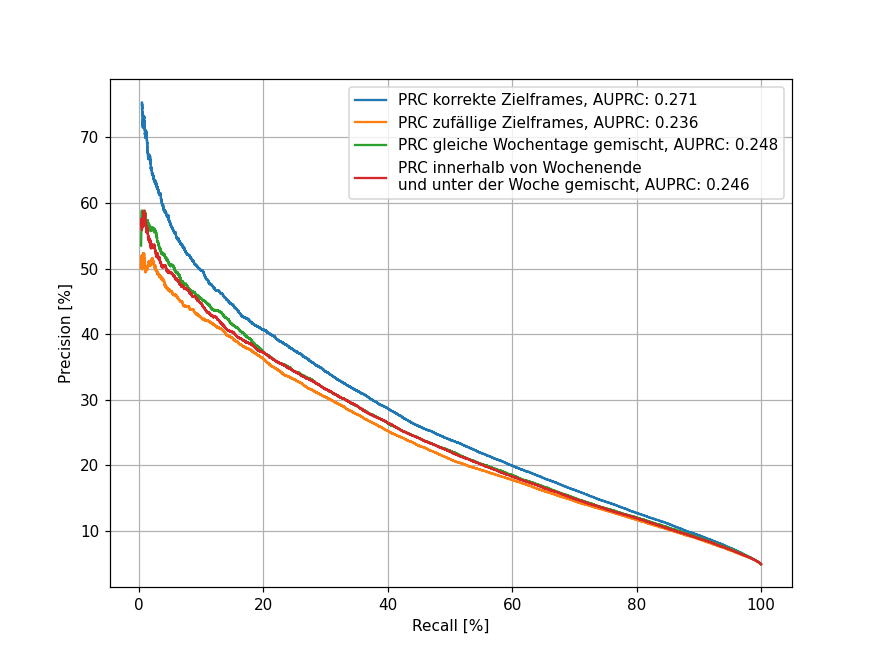
\includegraphics[width=1.0\textwidth,height=12cm,keepaspectratio=true]{content/images/PRCValGetrennt.png}
    \caption{\acrshortpl{prc} und \acrshort{auprc}-Werte mit wahren und gemischten Zielframes}
    \label{fig:PRCValGetrennt}
\end{figure}

Hierbei ist anzumerken, dass die \acrshortpl{prc} den Durchschnitt des gesamten Validierungsdatensatzes darstellen und nicht wie in \autoref{fig:PredExGraphsPRC} nur eine einzelne Vorhersage.
Dadurch verlaufen die Kurven weicher und gleichmäßiger.
Es ist deutlich zu erkennen, dass die mit den zufälligen Zielframes erzeugte \acrshort{prc} (orange) am niedrigsten liegt und auch den geringsten \acrshort{auprc}-Wert von 0,236 aufweist.
Die \acrshort{prc} mit den korrekten Zielframes liegt hingegen höher.
Dadurch erfährt auch der \acrshort{auprc}-Wert einen Zuwachs von ca. 15\,\% und liegt somit bei 0,271.

Im vorherigen Abschnitt wurde bereits aufgezeigt, dass das Modell den Unterschied zwischen Wochenende und unter der Woche gut erlernen kann.
Dieser Unterschied ist jedoch sehr einfach zu erkennen, da es am Wochenende durchschnittlich nur halb so viele Radarkontrollen gibt wie unter der Woche.
Daher ist es für die Evaluierung interessant, diesen Effekt bei der Analyse auszuschließen.
Dies kann realisiert werden, indem nur die Samstage und Sonntage untereinander gemischt werden, wie auch die Tage Montag bis Freitag.
Es kann auch noch einen Schritt weiter gegangen werden, indem nur gleiche Wochentage gemischt werden.
Hierdurch werden jedoch u.\,U. wochentagabhängige Muster unterdrückt, die eine durchaus valide Leistung des Modells darstellen.
Andererseits kann mit diesem Vorgehen untersucht werden, ob überhaupt wochentagabhängige Muster in den Daten existieren.
Daher sind in \autoref{fig:PRCValGetrennt} beide Ansätze dargestellt.
Es ist erkennbar, dass die Kurven wie erwartet etwas über der Kurve der komplett zufälligen Zielframes liegt.
Daraus kann abgeleitet werden, dass das Modell tatsächlich den Unterschied zwischen Wochenende und unter der Woche gelernt hat.
Jedoch liegen die Kurven immer noch deutlich unter der Kurve der korrekten Zielframes.
Daraus folgt, dass es im Datensatz noch weitere Muster gibt, die über den Unterschied zwischen Wochenende und unter der Woche hinaus gehen und dass die gewählte Modellarchitektur fähig ist, diese zu erlernen.
Bei den Kurven ist besonders der linke Rand interessant, da dies der Bereich ist, in dem sich das Modell mit den Vorhersagen sehr sicher ist.
Daher ist dieser Bereich in \autoref{fig:PRCValGetrenntZoom} vergrößert dargestellt.

\begin{figure}[h]
    \centering
    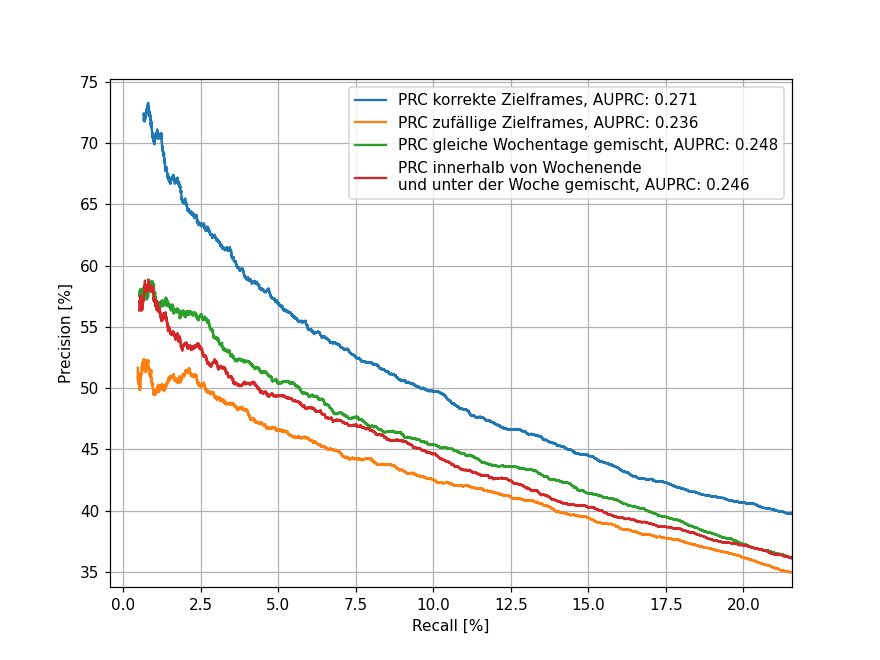
\includegraphics[width=1.0\textwidth,height=12cm,keepaspectratio=true]{content/images/PRCValGetrenntZoom.png}
    \caption{\acrshortpl{prc} im Detail bei geringen Recall- und hohen Precision-Werten}
    \label{fig:PRCValGetrenntZoom}
\end{figure}

Der dargestellte Bereich entspricht einer Perzentilgrenze von etwa 96\,\% am rechten Rand bis 99,5\,\% am linken Rand.
Hier bestätigt sich die Vermutung, dass es wochentagabhängige Muster in den Daten gibt, da die grüne Kurve, für die nur gleiche Wochentage gemischt wurden, etwas über der roten Kurve liegt.
Die Signifikanz dieses Unterschieds ist jedoch diskutabel.
Zusammenfassend bestätigt die durchgeführte Evaluierung, dass es verschiedene Muster in den Daten gibt und dass das Modell dazu in der Lage ist, diese Muster zu erlernen.
